\documentclass{standalone}
\usepackage{tikz}
\usetikzlibrary{positioning}
\usetikzlibrary{mindmap,trees}
\usepackage{verbatim}

\begin{document}
\pagestyle{empty}
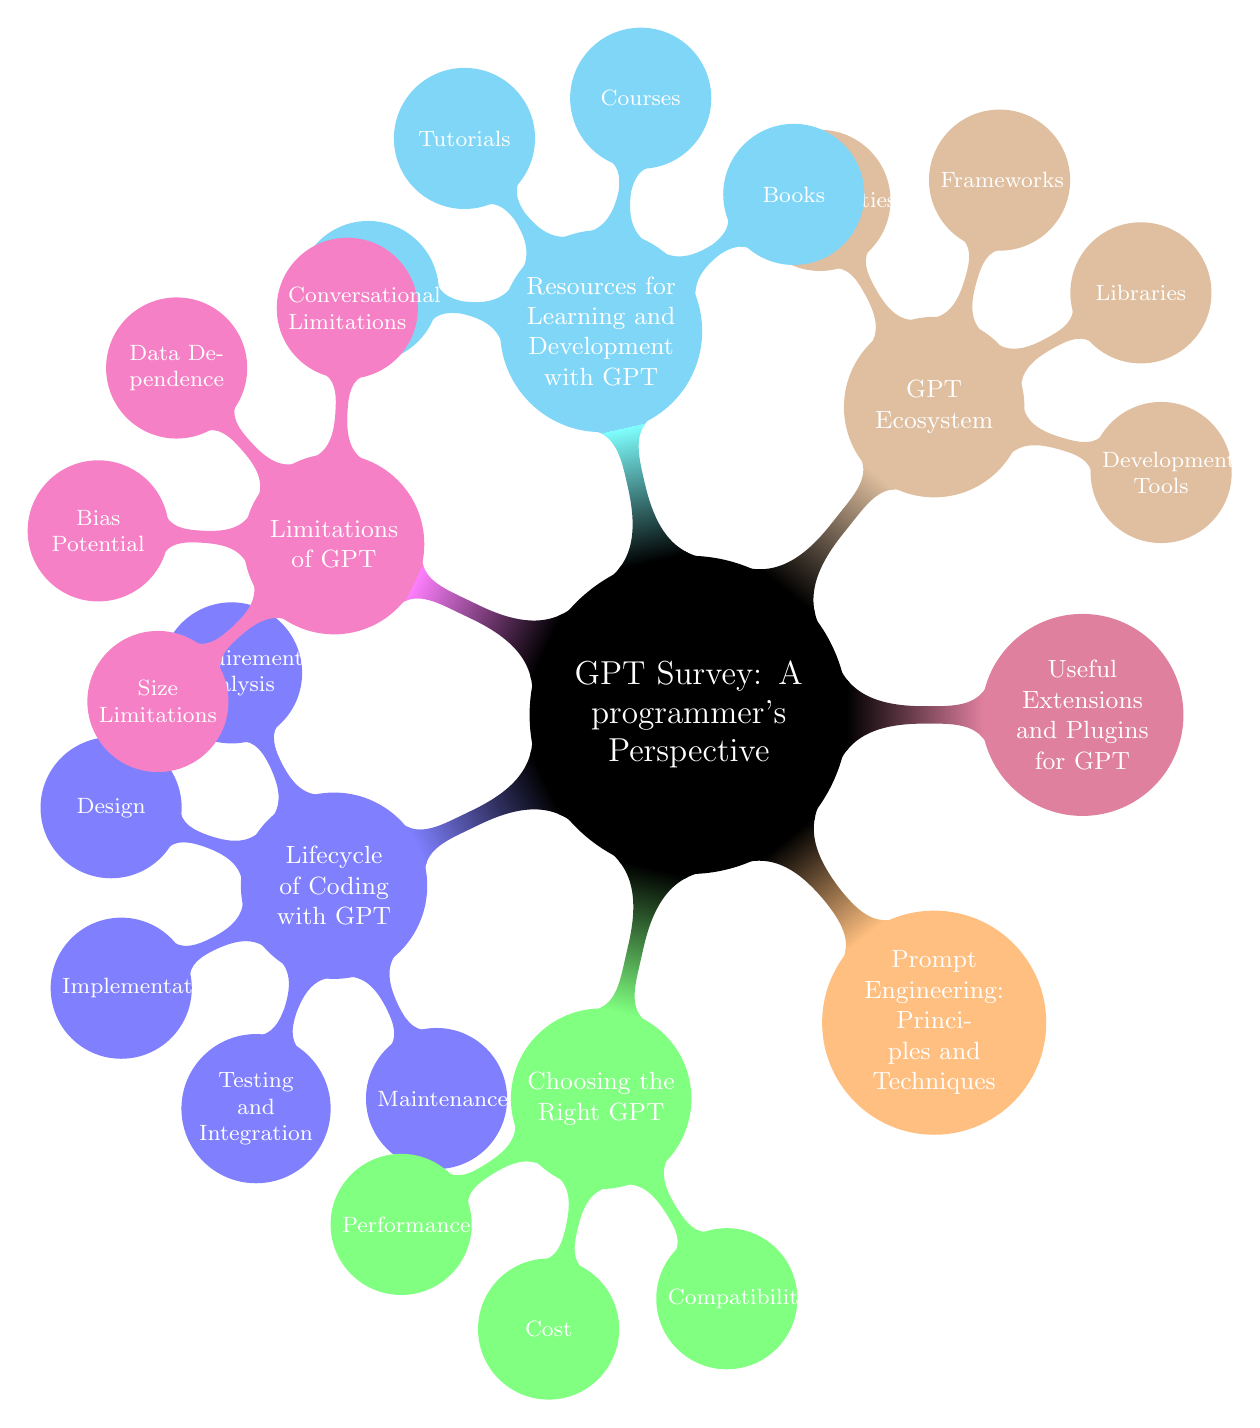
\begin{tikzpicture}[mindmap, grow cyclic, every node/.style=concept, concept color=black, text=white,
  level 1/.append style={level distance=5cm, sibling angle=360/\the\tikznumberofchildren},
  level 2/.append style={level distance=3cm, sibling angle=45},
]

  \node {GPT Survey: A programmer's Perspective}
    child[concept color=blue!50] { node {Lifecycle of Coding with GPT}
      child foreach \y in {
        {Requirement Analysis},{Design},{Implementation},{Testing and Integration},{Maintenance}
      } {
        node[concept] {\y}
      }
    }
    child[concept color=green!50] { node {Choosing the Right GPT}
      child foreach \y in {
        {Performance},{Cost},{Compatibility}
      } {
        node[concept] {\y}
      }
    }
    child[concept color=orange!50] { node {Prompt Engineering: Principles and Techniques}}
    child[concept color=purple!50] {node {Useful Extensions and Plugins for GPT}}
    child[concept color=brown!50] { node {GPT Ecosystem}
      child foreach \y in {
        {Development Tools},{Libraries},{Frameworks},{Communities}
      } {
        node[concept] {\y}
      }
    }
    child[concept color=cyan!50] {
        node[concept] (n) {Resources for Learning and Development with GPT}
        child foreach \y in {
          {Books},{Courses},{Tutorials},{Blogs}
        } {
          node[concept] {\y}
        }
    }
    child[concept color=magenta!50] {
        node[concept](o){Limitations of GPT}
        child foreach \y in {
          {Conversational Limitations},
          {Data Dependence},
          {Bias Potential},
          {Size Limitations}
        } {
          node[concept] {\y}
        }
    };
\end{tikzpicture}
\end{document}